\chapter{Related Work}

 Related work that had a direct or influencing impact on the design and implementation of this master's thesis' work is analyzed in this Chapter including topics such as, single sign-on (SSO), the Security Assertion Markup Language (SAML), the Shibboleth project, the SWITCH edu-ID identity provider, the Corda distributed ledger (DL)  and the Corda accounts library \cite{shib-website},  \cite{eduid-website}, \cite{corda-website}, \cite{corda-accounts-library}. 

\section{Swiss Educhain Previous Work}

The work for Swiss Educhain is based on the preliminary work conducted by Jerinas Gresch in \cite{Gres18}, where a detailed analysis of the diploma issuance process in UZH was performed. The high-level requirements, the stakeholders and a high-level architecture with a working proof-of-concept (PoC) was the produced outcome. Through this, the formalized proposal for the Swiss Educhain project came to fruition \cite{educhain-proposal} with a more technical architecture \cite{educhain-architecture}. The work for the Swiss Educhain service in this thesis, which is in close collaboration with the work in \cite{mueller20}, considers previous work but follows a greenfield approach not constrained by any previous assumptions or decisions. The main aim is to design and create an end-to-end digital service that also encapsulates the digital issuance of a diploma, in contrast with previous work where diploma issuance is designed to occur in the legacy system. More information on the design and implementation of the Swiss Educhain service is provided in Chapters \ref{ch:design} and \ref{ch:implementation}.  


\section{SWITCH} \label{sec:switch-related-work}

SWITCH is a Swiss foundation that provides a variety of information technology services to the academic community, mainly in the areas of network, security and identity management \cite{switch-foundation-about}. The identity management offerings, namely SWITCHaai (Authentication and Authorization Infrastructure) and SWITCH edu-ID, provide access to academic services in a secure manner \cite{switch-services-aai-eduid}. The relationship between SWITCH, SWITCHaai and SWITCH edu-ID as part of the federation \cite{switch-federation} is depicted in Figure \ref{fig:switch-federation}.

\begin{figure}[ht!]
	\centering
	\captionsetup{width=.7\linewidth}
	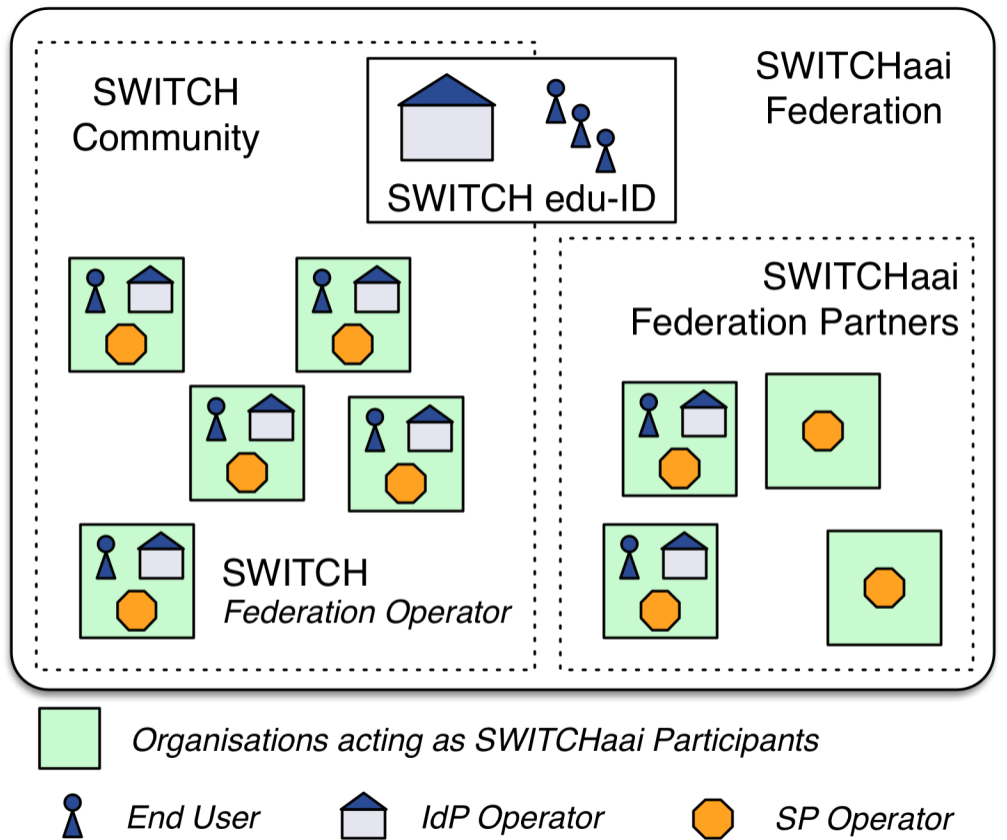
\includegraphics[width=0.55\textwidth]{figs/ch3/switch-federation}
	\caption{SWITCH identity federations \cite{eduid-service-description}.}
	\label{fig:switch-federation}
\end{figure}

\subsection{SWITCH edu-ID} \label{ssec:switch-eduid}

SWITCH edu-ID is the logical evolution of SWITCHaai and will eventually replace it as the single identity solution across academic organizations and services in Switzerland. SWITCH edu-ID builds upon existing infrastructure and leverages the SWITCHaai wide adoption and backwards compatibility. Several advantages for organizations, services and users make the adoption of SWITCH edu-ID attractive \cite{switch-eduid-benefits}: 

\begin{description}
	\itemsep0em
	\item \textbf{Organizations} 
		\begin{description}
			\itemsep0em
			\item Organizations don't need to operate an own IdP (Identity Provider).
			\item Covers also guests, not only regular students and collaborators.
			\item Organizations can realize their one-identity-concept.
			\item Organizations and their users keep the control over their data.
			\item Organizations can use features implemented once and at one place. \cite{eduid-for-organizations}
		\end{description}
	\item \textbf{Services}
		\begin{description}
			\itemsep0em
			\item High security (SWITCHaai basis, controlled guidelines and high-quality attributes).
			\item Less administration effort.
			\item Compatibility with SWITCHaai, Switzerland and internationally. \cite{eduid-for-services}
		\end{description}
	\item \textbf{Users}
		\begin{description}
			\itemsep0em
			\item One identity for all academic services, lifelong, user-controlled and secure.
			\item Simple and safe to use with transparent data quality and forwarding. \cite{eduid-for-users}
		\end{description}
\end{description}

From a technical point of view, SWITCH edu-ID aims to make a shift from a role-based to a \textbf{persistent identity} model, with one long-living digital identity for the user. A user has more control over their data, and the responsibility to provide accurate data and to verify fields of the account individually, a visual representation of the user account in SWITCHaai and SWITCH edu-ID is shown in Figure \ref{fig:eduid-user-attr}. A user who is no longer member of a university and has no other affiliation(s) retains the private, user managed part of a SWITCH edu-ID identity \cite{eduid-architecture}.

\begin{figure}[H]
	\centering
	\captionsetup{width=\linewidth}
	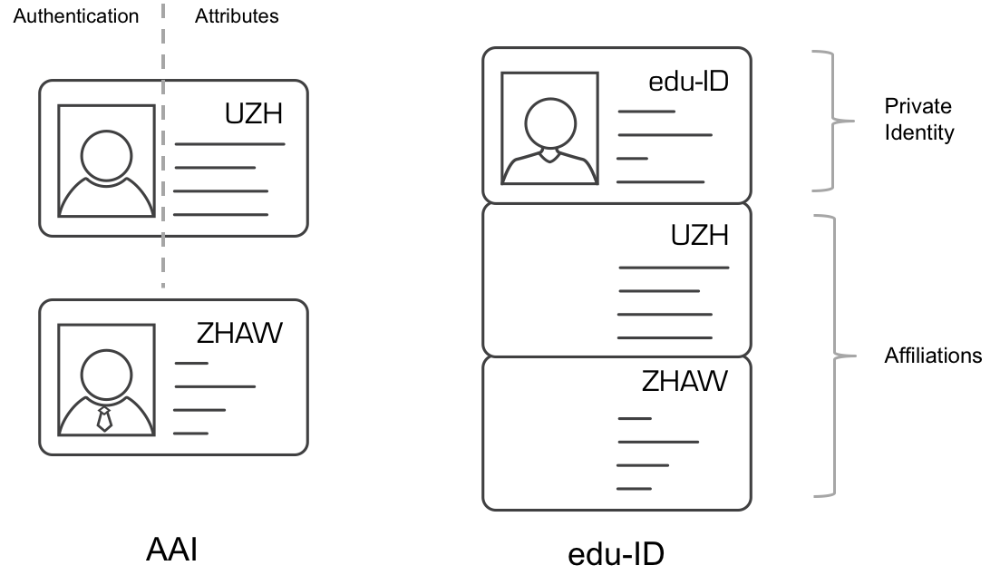
\includegraphics[width=0.6\textwidth]{figs/ch3/eduid-vs-aai}
	\caption{User account structure with two affiliations, compared in aai and edu-ID \cite{eduid-architecture}.}
	\label{fig:eduid-user-attr}
\end{figure}

The authentication functionality is delegated to the SWITCH edu-ID identity provider (IdP), which manages the accounts' lifecycle, and delivers the requested subset of attributes to different services. Universities will no longer be the identity providers, but will act as \textbf{attribute authorities} (AAs) and will assign roles and access rights to users through attribute values. This enables attribute aggregation for users with multiple affiliations and the users keep a persistent account independent to duration of their affiliation with an organization. A detailed technical comparison of SWITCH edu-ID and SWITCHaai is available in \cite{eduid-vs-aai}.

SWITCH edu-ID is operated by SWITCH and is built upon multiple components that offer different pieces of functionality as shown in the architecture diagram in Figure \ref{fig:eduid-architecture}. It is also tightly integrated with Swiss universities and academic institutions, but technically allows non-academic users and service providers to be part of the ecosystem as well. The most important notion in the SWITCH edu-ID ecosystem is the \textbf{affiliation} which determines the nature of the relationship between a user and one or more organizations. The user's edu-ID account can be created before or after an affiliation to an organization is linked and duplicate accounts are automatically detected (through the \texttt{matriculationNr} attribute which is unique per person across universities) and can be merged into one. 

\begin{figure}[h]
	\centering
	\captionsetup{width=.8\linewidth}
	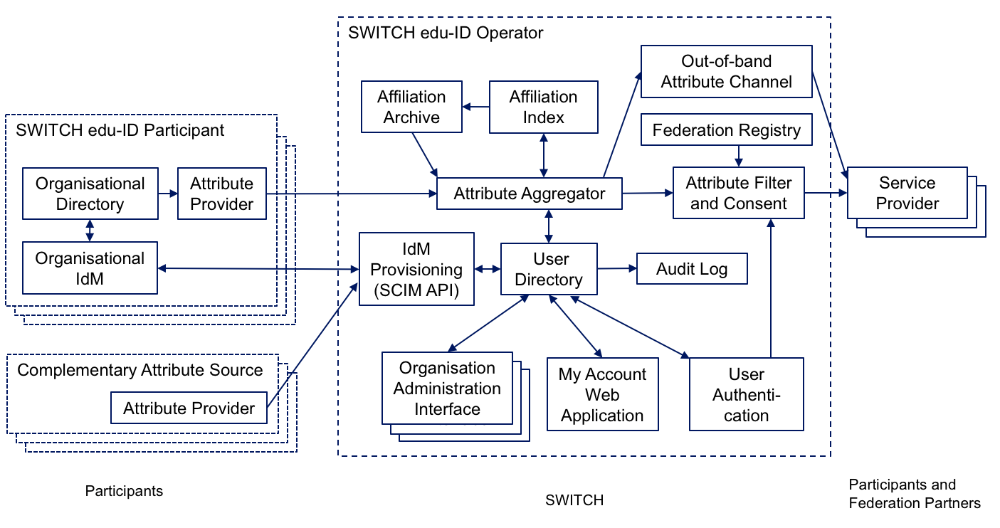
\includegraphics[width=0.9\textwidth]{figs/ch3/eduid-architecture}
	\caption{SWITCH edu-ID component architecture \cite{eduid-architecture}.}
	\label{fig:eduid-architecture}
\end{figure}

The Swiss Educhain is a Service Provider (SP) in the SWITCH edu-ID ecosystem and aims to provide a service initially to edu-ID users affiliated with UZH as students and later on to members of multiple organizations, details on the design and functionality are provided in Chapter \ref{ch:design}. To access a service, a user authenticates through the central edu-ID IdP. All the user managed attributes and the linked affiliation organizational attributes are collected by the aggregator, and only the ones requested by the service are chosen. Finally, after a user has given consent, the attributes are transmitted to the service \cite{eduid-architecture}.


\subsection{Shibboleth} \label{ssec:shibboleth-related-work}

Shibboleth is an open source software that implements the Security Assertion Markup Language (SAML) standard. It consists mainly of two major parts, an identity provider (IdP) and a service provider (SP). The most used scenario includes a third component, usually a web browser to complete a web single sign-on (SSO). A simple sequence diagram that shows the high-level steps of the web single sign-on process in Shibboleth is depicted in Figure \ref{fig:sso-diagram}. 

\begin{figure}[H]
	\centering
	\captionsetup{width=.8\linewidth}
	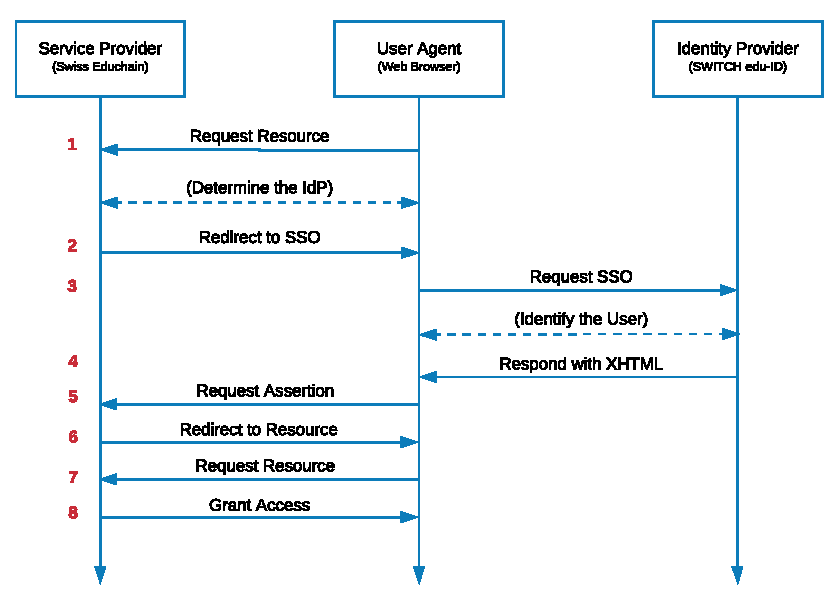
\includegraphics[width=0.8\textwidth]{figs/ch3/web-sso-diagram}
	\caption{Web single sign-on sequence diagram.}
	\label{fig:sso-diagram}
\end{figure} 

Shibboleth IdPs and SPs exchange authentication, authorization and configuration information between them securely via an (usually encrypted) xml metadata file. The IdPs and SPs in the metadata file typically form a federation similar to the ones visualized in Figure \ref{fig:switch-federation}. A federation is used to denote a trust relationship between the participating members. The security of messaging between IdP and SPs is handled through cryptography at various steps of the process. For example, SAML messages are usually digitally signed, and encrypted. \cite{sso-shibboleth-toronto}


\section{Corda} \label{sec:corda}

Corda is a distributed ledger technology platform that can be categorized as a private permissioned blockchain (in this context the term blockchain refers to Corda's terminology and not the technical term) according to the classification described in Section \ref{ch:background-blockchain}. Corda is offered as open source software \cite{corda-github}, developed and maintained mainly by R3 \cite{r3-website}, a dedicated enterprise blockchain software firm, along with additional contributions from the community \cite{corda-contributions}, \cite{corda-community}.

\begin{figure}[H]
	\centering
	\captionsetup{width=.8\linewidth}
	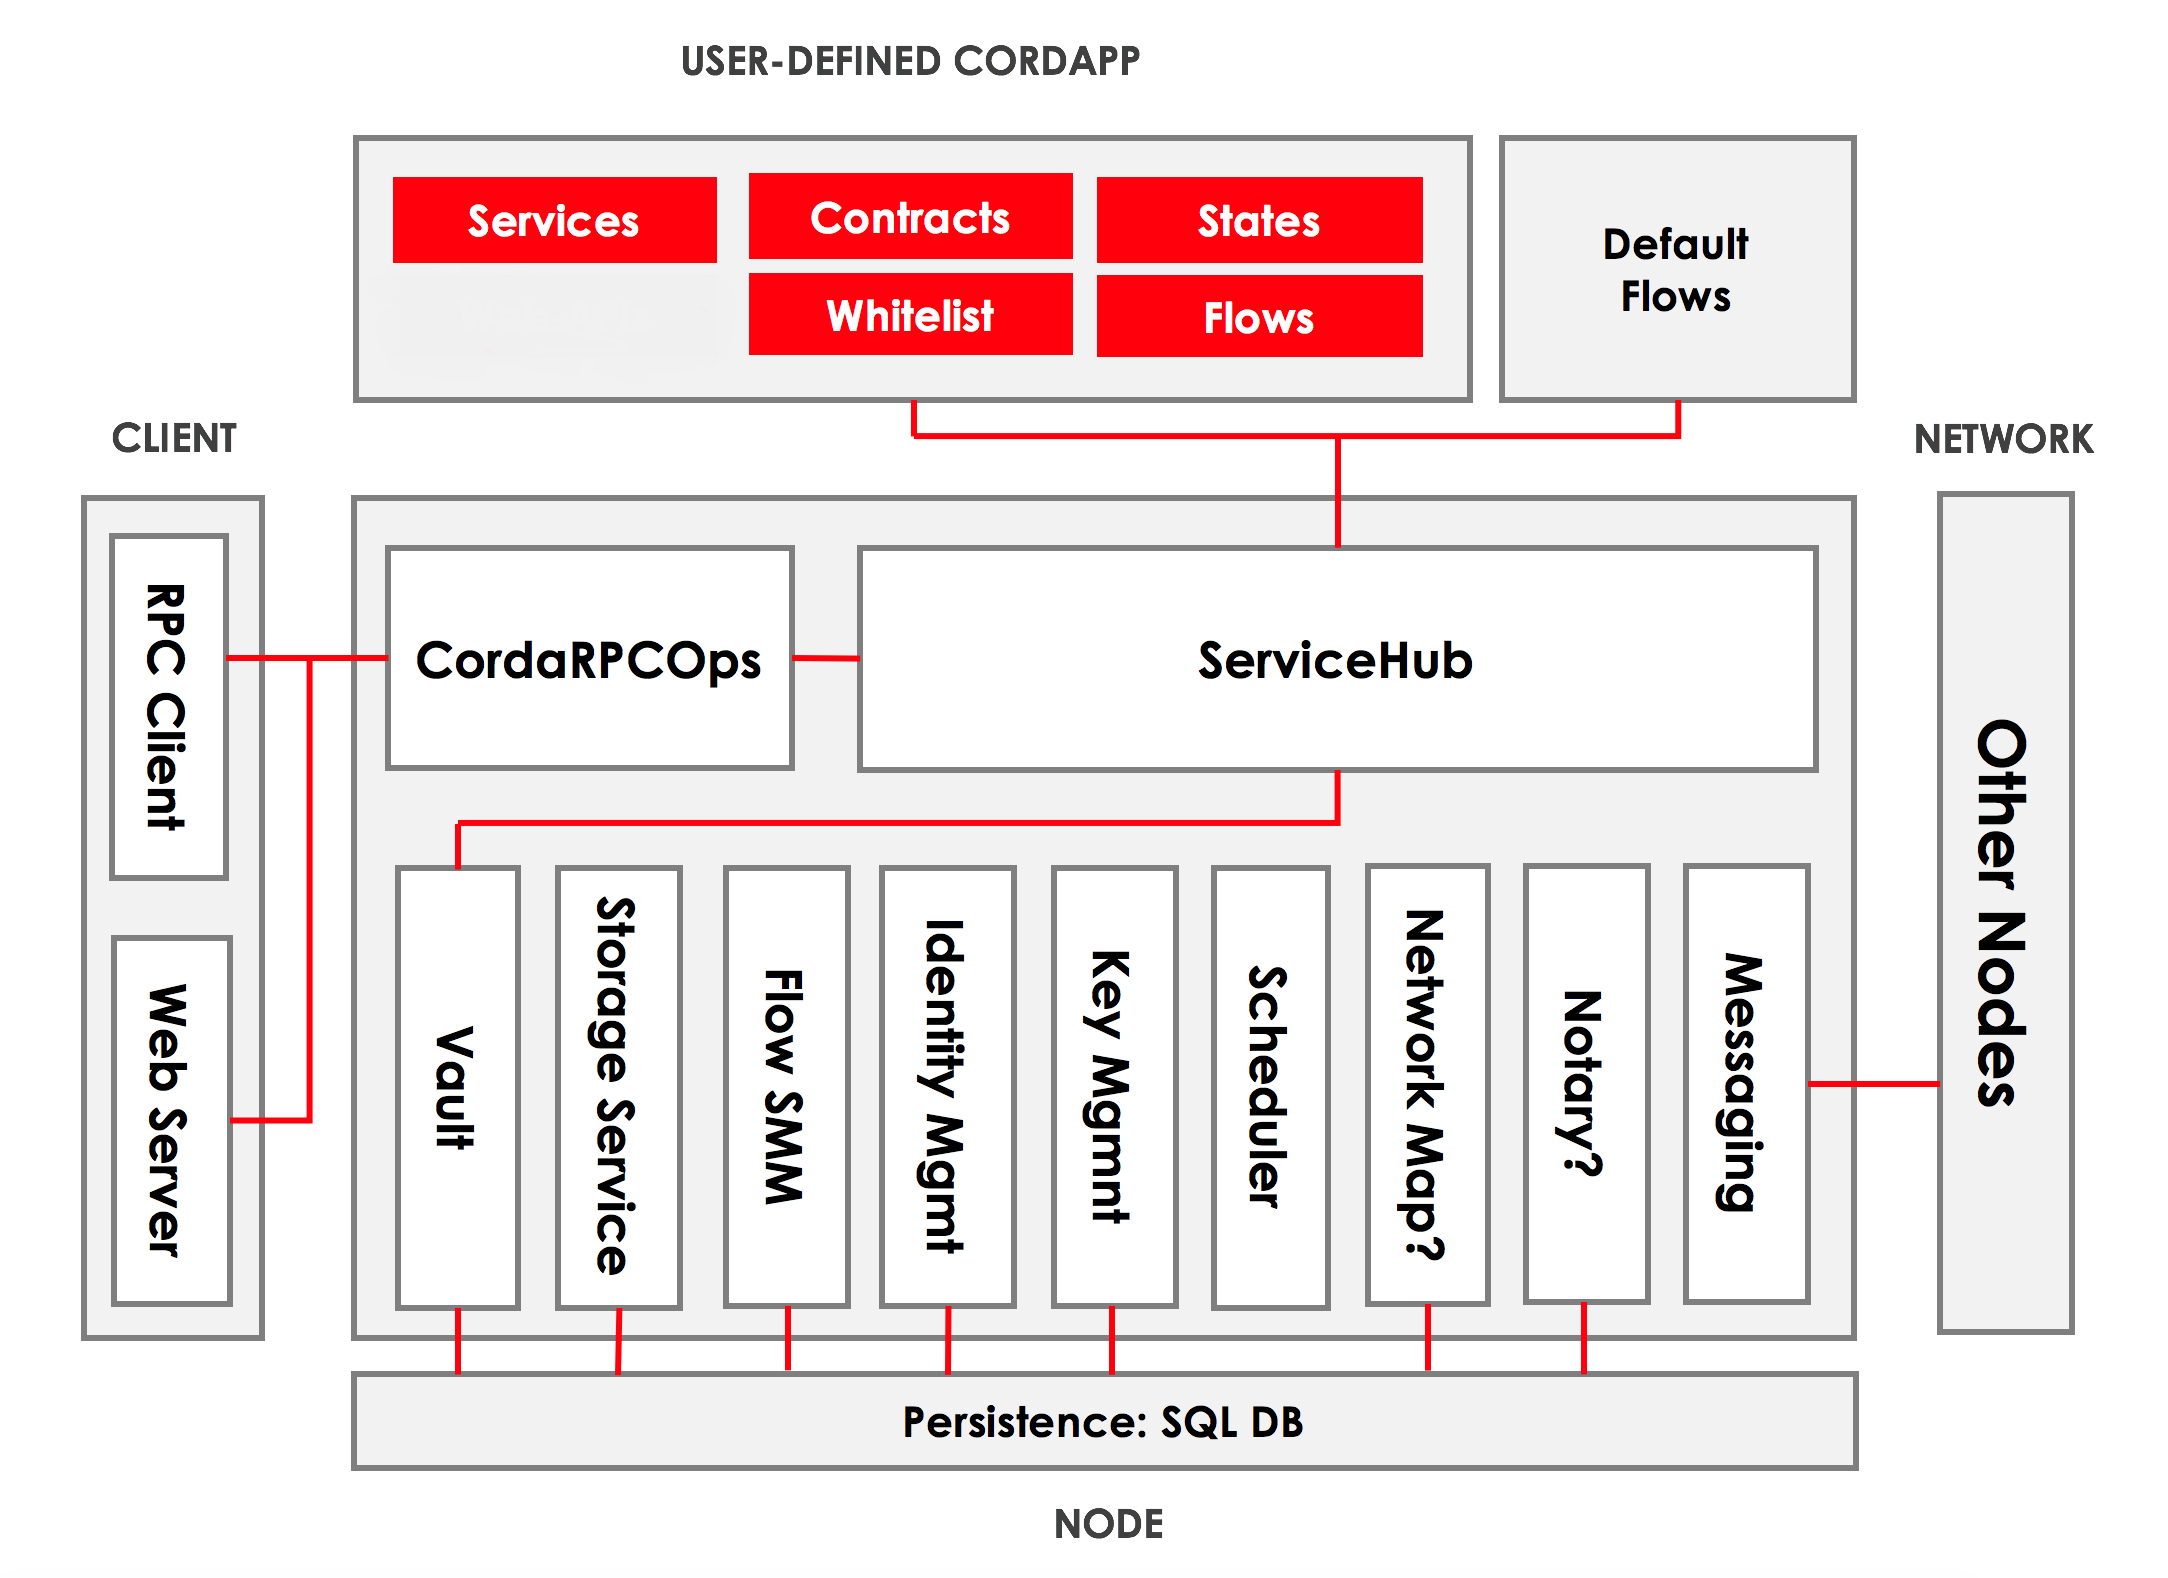
\includegraphics[width=0.8\textwidth]{figs/ch3/node-architecture}
	\caption{Corda node architecture \cite{corda-nodes}}
	\label{fig:node-architecture}
\end{figure} 


The Corda key concepts as identified in \cite{corda-concepts} and which are relevant to Swiss Educhain are shortly described:  
\begin{description}
	\itemsep0em
	\item\textbf{The network} - the ecosystem that Corda exists in.
	\item\textbf{The ledger} - the ledger, and how facts on the ledger are shared between nodes.
	\item\textbf{States} - the states represent shared facts on the ledger.
	\item\textbf{Transactions} - the transactions update the ledger states.
	\item\textbf{Contracts} - the contracts govern the ways in which states can evolve over time.
	\item\textbf{Flows}	- the flows describe the interactions that must occur to achieve consensus.
	\item\textbf{Whitelist} - the classes in the whitelist can be deserialized.
\end{description}

When one builds a custom Corda Decentralized Application (CorDapp), the CorDapp will have state, transaction, contract and flow classes. Nodes on the Corda network are instances that run the Corda DJVM (Deterministic JVM) \cite{corda-djvm} which can host one or more CorDapps simultaneously. Corda offers a lot of different pieces of functionality that run in the background in the form of services and are exposed to the CorDapps via the ServiceHub as depicted in Figure \ref{fig:node-architecture}.

Initially, R3 targeted financial institutions and business-to-business (B2B) transactions as the main use case for the platform. This naturally influenced Corda's design and functionality resulting in what is the main differentiating factor between Corda and other public or private blockchain platforms, it being the lack of a broadcast mechanism. This technically is translated in the existence of multiple smaller ledgers and the lack of a single global ledger in the network \cite{corda-network}. Corda uses a point-to-point messaging system instead of a gossiping mechanism, transaction data are only shared to the participants of a transaction, and sharing is performed only on a need-to-know basis. Notary might also gain access to the the data in order to be able to validate a transaction if needed, transactions can also be validated without access to any of the participants' data, depending on the type of transaction and contract rules \cite{corda-ledger}, \cite{corda-contracts}.

\subsection{Corda Accounts} \label{ssec:corda-accounts}

Until recently inside the Corda network identities, were mapped to a single deployed node instance, this design came from the original perception that the Corda network would be used for business-to-business (B2B) transactions between entities belonging to a certain business network. This assumed that each entity would be able to deploy and operate an own node, something that is not the case in most applications. After high demand from the community and to be able to offer competitive functionality, R3 introduced the Corda Accounts SDK (Software Development Kit) library \cite{corda-accounts-announcement} \cite{corda-accounts-library}.

\begin{figure}[ht]
	\centering
	\captionsetup{width=.8\linewidth}
	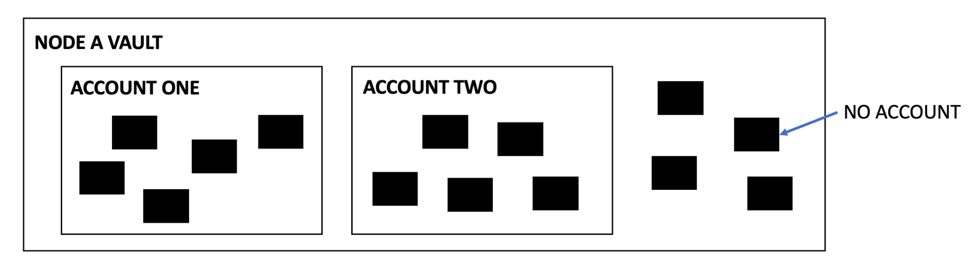
\includegraphics[width=0.6\textwidth]{figs/ch3/accounts-node}
	\caption{Account based node vault partition \cite{corda-accounts-library}.}
	\label{fig:accounts-node}
\end{figure} 

Accounts are a logical subset inside a node's vault as shown in Figure \ref{fig:accounts-node}. The vault can be described as a node's encrypted storage. Unlike the nodes, the accounts do not have a unique identifier at the network level, they inherit the node's CordaX500Name. Accounts need to be managed at the application level to make them identifiable and use them to represent different entities and transact. Figure \ref{fig:accounts-transactions} shows the different transaction options for accounts. Three different options exist, account-to-account transaction inside the same node, account-to-node transaction and account-to-account transaction between accounts that are hosted in different nodes.

\begin{figure}[H]
	\centering
	\captionsetup{width=.8\linewidth}
	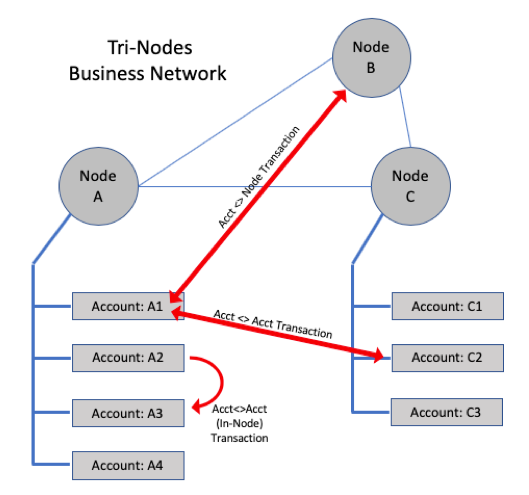
\includegraphics[width=0.55\textwidth]{figs/ch3/accounts-transactions}
	\caption{Account transaction types \cite{corda-accounts-library}.}
	\label{fig:accounts-transactions}
\end{figure} 

It is important to note that the Accounts library is not part of the main Corda release but can be optionally added as a dependency and used by a CorDapp. There is also the option to use accounts in some nodes of the network only, allowing for a hybrid setup. In the current Swiss Educhain service implementation only account-to-account transactions between accounts that reside in the same node are executed. A more detailed explanation on the design and implementation of application level accounts is provided in Chapters \ref{ch:design} and \ref{ch:implementation}.
